
\section{Related Work}
\label{sec:related_work}
\paragraph{Tool-using LLMs.} Despite strong reasoning and generation abilities, LLMs fall short on tasks requiring real-time access, accurate computation, or environment interaction, motivating the development of \emph{LLM-based agents} that leverage external tools. 
Representative examples include LLMs that use a web-browsing environment for question answering~\citep{nakano2022webgptbrowser}, a Python interpreter for arithmetic and symbolic reasoning~\citep{gao2023palprogramaidedlanguagemodels}, and information retrieval for grounding in dialogue~\citep{thoppilan2022lamdalanguagemodelsdialog}. 
The range of tools explored in the literature is far broader, and we refer readers to the comprehensive survey in~\citet{Qu_2025} for full coverage.

\paragraph{Synthetic agentic datasets.} While tool-using LLMs demonstrate the promise of agents, scaling their development requires large volumes of training data. To this end, recent efforts have introduced synthetic agentic datasets that emulate queries, tools, and environment feedback at scale \citep{patil2023gorillalargelanguagemodel,tang2023toolalpacageneralizedtoollearning,qin2023toolllmfacilitatinglargelanguage,zeng2023agenttuningenablinggeneralizedagent,xu2025toucan,li-etal-2023-api}. Gorilla~\citep{patil2023gorillalargelanguagemodel} uses a self-instruct approach to generate instruction–API pairs. ToolAlpaca~\citep{tang2023toolalpacageneralizedtoollearning} leverages a multi-agent simulation environment to build a diverse tool-use corpus, while ToolLLM~\citep{qin2023toolllmfacilitatinglargelanguage} employs ChatGPT to synthesize instruction–solution pairs involving real-world RESTful APIs. AgentTuning~\citep{zeng2023agenttuningenablinggeneralizedagent} adopts GPT-4 as an agent to generate trajectories across six task domains. API-Bank~\citep{li2023apibankcomprehensivebenchmarktoolaugmented} uses a multi-agent pipeline to generate domains, simulate APIs, construct queries, and validate responses. APIGen~\citep{liu2024apigenautomatedpipelinegenerating}, built on ToolBench~\citep{qin2023toolllmfacilitatinglargelanguage}, applies multi-stage verification with diverse prompt templates to ensure accuracy and coverage. ToolBridge~\citep{jin2024toolbridgeopensourcedatasetequip} curates a dataset of Python-based tool invocations via selection, conversion, and filtering of public corpora. BUTTON~\citep{chen2025facilitatingmultiturnfunctioncalling} generates multi-turn function-calling data with GPT-4o, combining bottom-up task evolution with top-down decomposition of complex tasks. Finally, ToolACE~\citep{liu2025toolacewinningpointsllm} introduces a pipeline for synthesizing diverse, complex, and accurate function-calling data through iterative tool evolution, complexity-guided dialog synthesis, and dual-layer verification.

Existing synthetic datasets have made significant progress in enabling tool-augmented LLMs, introducing diverse APIs, generation pipelines, and verification strategies. Our work takes a complementary direction: we simulate complete end-to-end trajectories that integrate reasoning steps, tool use, and environment feedback. This benchmark-agnostic design allows synthetic data to be extended across diverse domains and tasks, providing a flexible way to augment existing datasets with richer, trajectory-level supervision. In this sense, our method does not replace prior efforts but instead offers a means of extending their coverage and contributes agentic training.

\section{Experiment Setup}
\label{Detailed Experiment Setup}


\subsection{Supervised Fine-tuning}
\label{SFT Setup}


Our model SFT is conducted using LLaMA-Factory \citep{zheng2024llamafactory}, on a server with eight NVIDIA A100-SXM4-80GB GPUs. We follow \cite{prabhakar2025apigen} for the training parameters.
Table \ref{tab: training-hyperparameters} lists hyper-parameters for full parameter supervised fine-tuning. 


\begin{table}[!h]
\small
\centering
\caption{Hyper-parameters used for full parameter supervised fine-tuning.}
\resizebox{0.8\columnwidth}{!}{
\begin{tabular}{ll}
\toprule
\textbf{Hyper-parameter} & \textbf{Value} \\ \midrule
Learning Rate & $5 \times 10^{-6}$ \\
Number of Epochs & $2$ \\
Number of Devices & $8$ \\
Per-device Batch Size & $2$ \\
Optimizer & \texttt{Adamw} \\
Learning Rate Scheduler & \texttt{cosine} \\
Max Sequence Length  & $16384$ \\ \bottomrule
\end{tabular}
}
\label{tab: training-hyperparameters}
\end{table}


\subsection{GRPO}
\label{Grpo Setup}

We use the following hyper-parameters detailed in Table \ref{tab: rl hyperparameters} for RL training on the simulated environment. We perform experiments on eight A100 GPUs. The model is trained using RAGEN \citep{ragen}and VeRL \citep{sheng2024hybridflow}. The RL training is configured with a rollout of 16, 64 training steps, a maximum context length of 12,000 tokens, and up to 40 interaction rounds per task, with a temperature setting of 0.7. 

\begin{table}[htbp]
\small
\centering
\caption{Hyper-parameters for RL training.}
\begin{tabular}{ll}
\toprule
\textbf{Hyper-parameter} & \textbf{Value} \\ \midrule
Learning Rate & $1 \times 10^{-6}$ \\
Number of Steps & $64$ \\
Number of Devices & $8$ \\
Temperature & 0.7 \\
Top P & 1.0 \\
PPO Mini Batch Size & 32 \\
Max Response Length & $16384$ \\
KL Coefficient & $0.001$ \\
Rollout Engine & $\textsc{vllm (v0.8.2)}$ \\
Optimizer & \texttt{Adamw} \\
Learning Rate Scheduler & \texttt{cosine} \\
Warmup Ratio & $0.1$ \\
Agent Max Turn & 25 \\
Agent Max Action Per Turn & 1 \\
Clip Ratio High & 0.28 \\

\bottomrule
\end{tabular}
\label{tab: rl hyperparameters}
\end{table}




\section{Full Prompt for Synthetic Trajectory Generation}
\label{appendix:prompt}

See figure \ref{fig:Prompt to synthesize APIGen-MT} for synthesize APIGen-MT and Agenttuning, and see figure \ref{fig:Prompt to synthesize OfficeBench} for OfficeBench.




\begin{figure*}[htbp]
    \centering
\begin{tcolorbox}[title=Prompt to synthesize APIGen-MT and Agenttunig]
\begin{tcblisting}{
  title=,
  listing only,
  breakable,
  enhanced,
  colback=white,
  colframe=black!15,
  boxrule=0.3pt,
  listing options={
    basicstyle=\ttfamily\scriptsize, % ← 比 footnotesize 更小
    breaklines=true,
    columns=fullflexible
  }
}
You are an AI assistant that generates multi-turn conversation data for agent training. Your task is to create new agent trajectories based on existing examples.

## Example Trajectory:
{sample_text}

## Available Tools:
{available_tools}

CRITICAL FORMAT PRESERVATION REQUIREMENTS - ABSOLUTE COMPLIANCE:
1. **STRICTLY PRESERVE ORIGINAL FORMAT**: You MUST maintain the EXACT format structure from the example trajectory (EXCEPTION: function_call turns may include <think> tags when reasoning is needed)
2. **NO SYSTEM PROMPT GENERATION**: Do NOT generate any SYSTEM messages - follow the system prompt from the original example and that will be preserved separately
3. **TOOL CONSTRAINT ADHERENCE**: You MUST STRICTLY use ONLY the tools listed in the "Available Tools" section above. DO NOT use any tools outside this specified allowed tool set. This is MANDATORY.
4. **FORMAT CONSISTENCY**: Maintain identical conversation structure, role naming conventions, and response patterns as shown in the example (EXCEPTION: function_call turns may include <think> tags when reasoning is added)
5. **TURN COUNT MATCHING**: Generate approximately the SAME NUMBER of conversation turns as the example trajectory - the generated conversation should have a comparable length and depth to the sample data

## FUNCTION_CALL TURN REQUIREMENTS:
1. **REASONING IN THINK TAGS**: When making function calls, add brief reasoning (1-3 sentences) inside `<think> </think>` tags ONLY in FUNCTION_CALL turns after you output 'FUNCTION_CALL:'
2. **SELECTIVE REASONING**: Not every function call needs reasoning. Only include it when it helps explain the complex decision-making process
3. **STRICT TURN CONSTRAINT**: Reasoning in `<think> </think>` tags should ONLY appear in FUNCTION_CALL turns, NEVER in HUMAN, GPT, OBSERRVATION or additional turns
4. **FORMAT REQUIREMENT**: If reasoning is included, the FUNCTION_CALL turn are allowed to add the thinking sentences instead of only JSON format. You should follow this format:
'''
FUNCTION_CALL:
<think>
Brief reasoning about why this function call is needed (1-3 sentences). Ended with: I will call the function <function_name>.
</think>
{{"name": "function_name", "arguments": {{...}}}}
'''

## ABSOLUTE PROHIBITIONS:
- DO NOT use ANY tools that are not explicitly listed in the "Available Tools" section above
- DO NOT change the conversation format structure (human/gpt roles, value formatting, etc.) - EXCEPTION: function_call turns may include <think> tags when reasoning is needed
- DO NOT violate any fixed formatting elements, tool specifications, or requirements in system instructions from the example - EXCEPTION: function_call turns may include <think> tags when reasoning is added
- DO NOT generate significantly fewer or more turns than the example trajectory
- DO NOT invent or create new tools - use ONLY the provided tools

## Requirements:
1. Generate a completely NEW scenario/task that is different from the example but requires similar problem-solving patterns
2. Create a multi-turn conversation between Human and Assistant that demonstrates systematic problem-solving
3. The conversation should show the agent's reasoning process and step-by-step approach
4. **Start directly with a HUMAN message - do not include the SYSTEM content**

## Output Format:
Generate the conversation:
HUMAN: [user message content]
ASSISTANT: [assistant reply content]
HUMAN: [user message content]
ASSISTANT: [assistant reply content]
HUMAN: [user message content]
ASSISTANT: [assistant reply content]
...(until the task is finished and the conversation is complete)
\end{tcblisting}
\end{tcolorbox}
\caption{Prompt to synthesize APIGen-MT and Agenttunig}
\label{fig:Prompt to synthesize APIGen-MT}
\end{figure*}




\begin{figure*}[htbp]
    \centering
\begin{tcolorbox}[title=Prompt to synthesize OfficeBench]
\begin{tcblisting}{
  title=,
  listing only,
  breakable,
  enhanced,
  colback=white,
  colframe=black!15,
  boxrule=0.3pt,
  listing options={
    basicstyle=\ttfamily\scriptsize, % ← 比 footnotesize 更小
    breaklines=true,
    columns=fullflexible
  }
}
You are an AI assistant that generates multi-turn conversation data. Based on the provided example conversation, create a new conversation that expands the task to use multiple apps in a natural workflow.

Example conversation:\{seed\_sample\}

Your task:
1. Analyze the example task
2. Create a new task that naturally extends this workflow to use multiple different apps
3. The new task should be realistic and make sense - don't force apps together artificially
4. New created task should be diverse 

Available Tools:
{availabel tools}

## CRITICAL REQUIREMENTS - AVOID COMMON ERRORS:

### Critical Error Pattern - Insufficient Path/Directory Validation:
**Root Cause: Failure to perform directory ls or mkdir validation before operations**
- **File Path/Directory Errors**: Working directory or data directory spelling, hierarchy does not match expectations, no prior checking or directory creation
- **Mandatory Operation**: Before any file operations, use ls to confirm current directory structure and file existence
- **Directory Creation**: If creating new directories, must first use mkdir -p to ensure directory exists

## Workflow Best Practices:
1. **File Discovery**: Use shell commands (ls, find) to discover actual file names before operations
2. **App Context**: Always switch\_app before using different app APIs
3. **Data Operations**: Count/filter accurately, verify each step, preserve headers
4. **File Creation**: Use proper app APIs (Excel: new_file, Word: new_document), NOT shell touch

Requirements:
1. Follow the same conversation format as the example (\#\#Task: format, <think> and <answer> structure)
2. Generate a completely new task - don't copy the example
3. Make sure the workflow feels natural and logical
4. DON'T specify exact file names in the task - let the workflow discover them with shell commands
5. Include app switching with "Successfully switched to app: [app\_name]. Available actions:" messages
6. End with finish\_task action

Create a conversation that shows the complete workflow from start to finish with proper error prevention.

Please generate the conversation content directly in this format:
HUMAN: [human message content]
GPT: [GPT reply content]
HUMAN: [human message content] 
GPT: [GPT reply content]
... 

\end{tcblisting}
\end{tcolorbox}
\caption{Prompt to synthesize OfficeBench}
\label{fig:Prompt to synthesize OfficeBench}
\end{figure*}


\section{Full Prompt for RL on the simulated environment}
\label{appendix:prompt_rl}
Please see Figure \ref{fig:Prompt to simulated OfficeBench Environment Feedback} for prompt to simulated RL environment feedback and Figure \ref{fig:Prompt to compute OfficeBench RL Reward} for the prompt to compute the reward.

\begin{figure*}[htbp]
    \centering
\begin{tcolorbox}[title=Prompt to simulated OfficeBench Environment Feedback]
\begin{tcblisting}{
  title=,
  listing only,
  breakable,
  enhanced,
  colback=white,
  colframe=black!15,
  boxrule=0.3pt,
  listing options={
    basicstyle=\ttfamily\scriptsize, % ← 比 footnotesize 更小
    breaklines=true,
    columns=fullflexible
  }
}
You are an office environment simulator that needs to generate realistic environment feedback based on eval model's actions.

Current application: {self.current_app or "None selected"}

Available applications and action formats:
{action_formats}

{response_guidance}

Testbed Data of the task:
{testbed_text}

Please simulate the execution result of this action. You need to:
1. FIRST check if the action is valid according to the available action formats above
2. If the action is invalid (wrong app, wrong action name, missing parameters), return failure immediately. 
3. If valid, simulate realistic execution results
4. Return appropriate observation results

IMPORTANT: Only actions listed in the "Available applications and action formats" section are valid. If the action is not in that list, it should fail.

Response format:
```json
{{
    "success": true/false,
    "observation": "Specific observation result explaining success or failure."
}}
Please ensure your response is realistic. Invalid actions should always return success=false.

Current Task:
{current_task}

Previous history of the eval model's actions:
{self._get_interaction_history()}

Action to simulate:
{eval_context}
"""
\end{tcblisting}
\end{tcolorbox}
\caption{Prompt to simulate OfficeBench Environment Feedback}
\label{fig:Prompt to simulated OfficeBench Environment Feedback}
\end{figure*}


\begin{figure*}[htbp]
    \centering
\begin{tcolorbox}[title=Prompt to compute OfficeBench RL Reward]
\begin{tcblisting}{
  title=,
  listing only,
  breakable,
  enhanced,
  colback=white,
  colframe=black!15,
  boxrule=0.3pt,
  listing options={
    basicstyle=\ttfamily\scriptsize, % ← 比 footnotesize 更小
    breaklines=true,
    columns=fullflexible
  }
}
You need to evaluate whether the eval model has successfully completed the given task based on the interaction history.

Complete interaction history:
{interaction_history}

Please analyze the above information and determine whether the model has successfully completed the task based on the trajectory history and whether the final outcome meets the requirements if following all the actions. Do NOT simply judge success based on whether the model claimed "task finished". 

Please provide judgment in the following format:
```json
{{
    "reasoning": "Detailed explanation of your judgment about whether the task is successfully completed",
    "evidence": "Key evidence from the interaction history that supports your judgment",
    "task_success": true/false,
    "confidence": 0.0-1.0
}}
\end{tcblisting}
\end{tcolorbox}
\caption{Prompt to compute OfficeBench RL Reward}
\label{fig:Prompt to compute OfficeBench RL Reward}
\end{figure*}



\begin{figure*}[htbp]
    \centering
\begin{tcolorbox}[title=Prompt to simulate APIGen-MT Environment Feedback]
\begin{tcblisting}{
  title=,
  listing only,
  breakable,
  enhanced,
  colback=white,
  colframe=black!15,
  boxrule=0.3pt,
  listing options={
    basicstyle=\ttfamily\scriptsize,
    breaklines=true,
    columns=fullflexible
  }
}
You are a simulation environment. Based on the RL model's response, you need to simulate the human or tool response.
System prompt (task description and rules):
{self.system_prompt}
Reference conversation examples (use this as reference data):
{ref_conv_text}
Current conversation history:
{history_text}
RL model's latest response:
{agent_message}
Requirements:
1. Based on the reference conversation and system prompt, determine how to respond
2. **Important for tool call format checking**: 
   - If the RL model is attempting to call a tool, check if it is properly wrapped in <tool_call></tool_call> tags
   - If the tool call is NOT in <tool_call> tags or has incorrect format (e.g., malformed JSON, wrong structure), return an error message like: "Error: Tool call must be wrapped in <tool_call></tool_call> tags with proper JSON format"
   - Only if the tool call format is correct, proceed to generate the tool response
3. **Important for tool responses**: 
   - If the RL model called a tool correctly, check if related results exist in the reference conversation
   - If YES: Include the related results from the reference conversation in the tool response
   - If NO: Generate reasonable results for the tool response based on the query parameters
   - If the format is incorrect, return an error message explaining why
3. If the RL model is waiting for human input, simulate the human's next message based on the reference conversation flow
4. Follow the pattern in the reference conversation examples, but adjust appropriately to fit the current conversation
5. If the task is completed or the conversation should end, output the "[TERMINATE]" marker
Output format:
- If continuing the conversation, output the message content directly
- If should end, output "[TERMINATE]"
Please directly generate the next message without the prefix "User/Tool response":
\end{tcblisting}
\end{tcolorbox}
\caption{Prompt to simulate APIGen-MT Environment Feedback}
\label{fig:prompt_simulate_environment_feedback}
\end{figure*}

\begin{figure*}[htbp]
    \centering
\begin{tcolorbox}[title=Prompt to compute APIGen-MT RL Reward]
\begin{tcblisting}{
  title=,
  listing only,
  breakable,
  enhanced,
  colback=white,
  colframe=black!15,
  boxrule=0.3pt,
  listing options={
    basicstyle=\ttfamily\scriptsize,
    breaklines=true,
    columns=fullflexible
  }
}
You need to evaluate the RL model's performance in this task and provide a reward.
System prompt (rules and policies):
{self.system_prompt}
Complete conversation history:
{history_text}
Evaluation criteria:
1. Did the RL model correctly understand the task requirements
2. Did the RL model follow the rules and procedures in the system prompt
3. **Tool call format check**: If the RL model attempted to call tools, were they properly wrapped in <tool_call></tool_call> tags with correct JSON format? If tool calls were malformed or not properly tagged, this should be considered a FAILURE.
4. Did the RL model handle tool responses correctly
**IMPORTANT**: 
- Simply completing the user's request is NOT sufficient if policies were violated
- Incorrect tool call format (missing <tool_call> tags or malformed JSON) should result in reward = 0
Output requirement:
Please output the evaluation result in JSON format:
{{
    "reasoning": "Detailed evaluation reasoning, explaining why this reward was given"
    "reward": 0 or 1,  // 0 means failure, 1 means success
}}
Please perform the evaluation:
\end{tcblisting}
\end{tcolorbox}
\caption{Prompt to compute APIGen-MT RL Reward}
\label{fig:prompt_compute_rl_reward}
\end{figure*}




\section{More Results of Synthetic Data}
\label{More Results of Synthetic Data}
\begin{figure*}
    \centering
    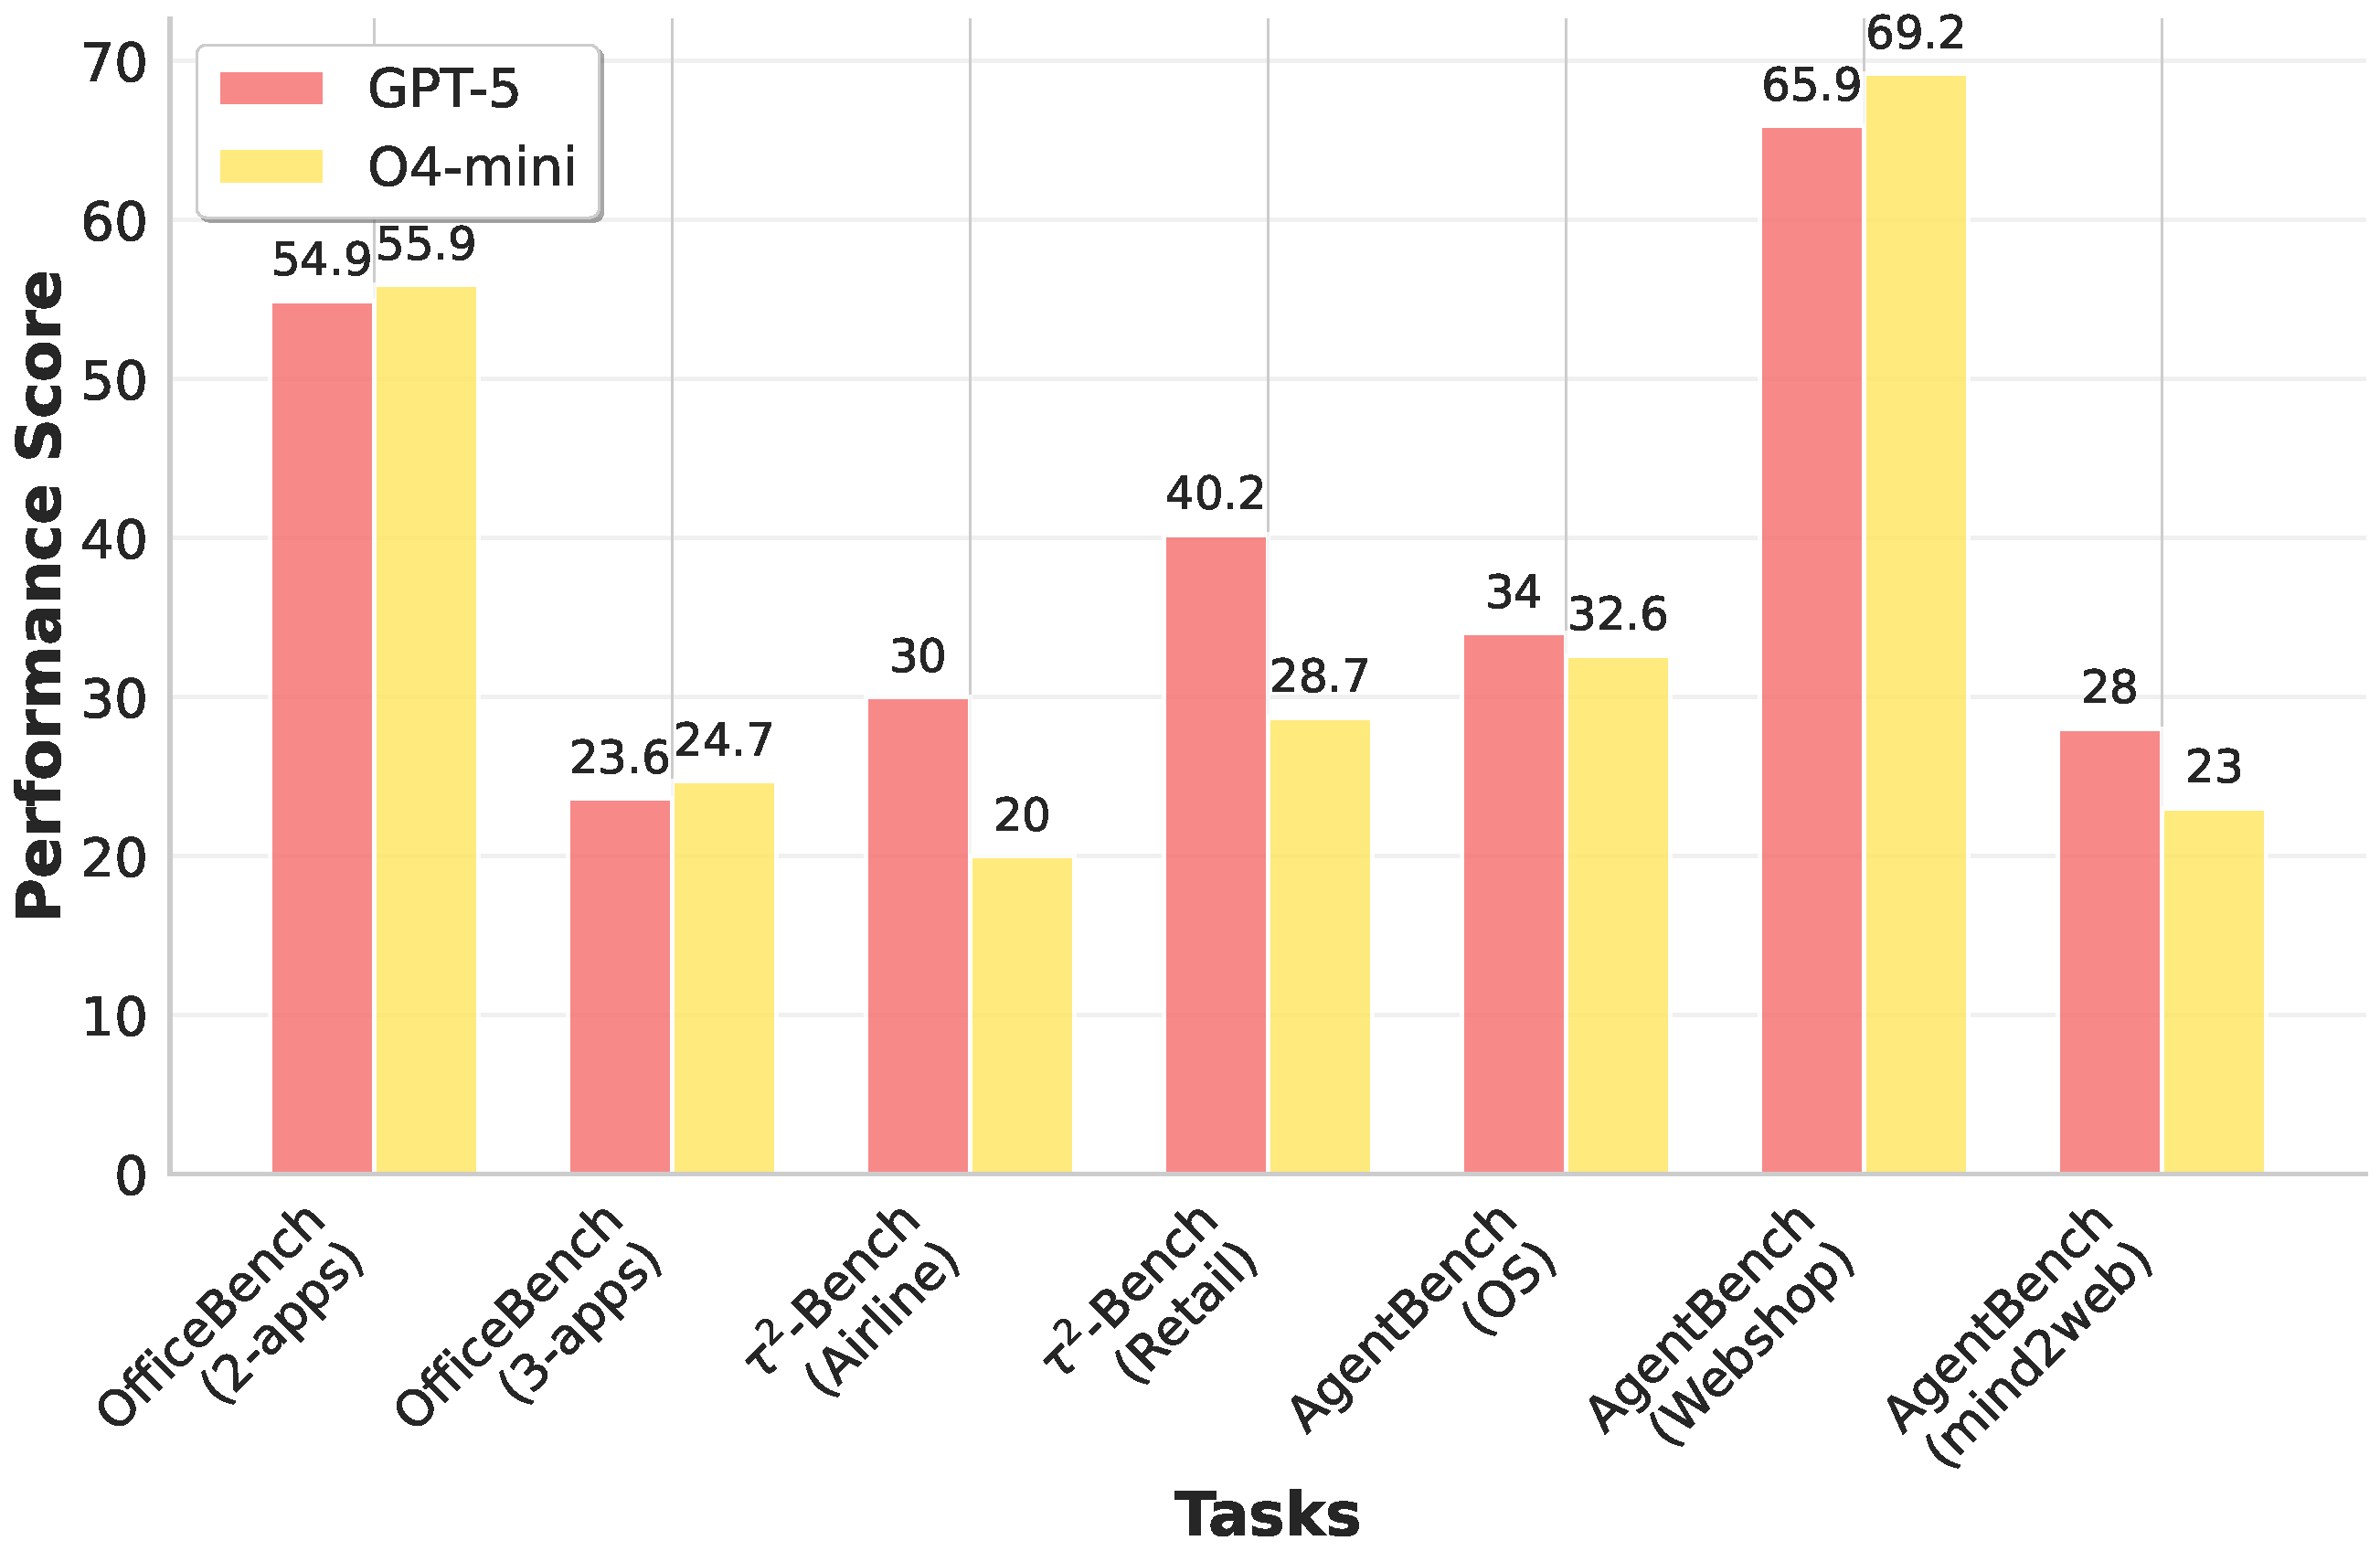
\includegraphics[width=0.6\textwidth]{figs/ablation_on_synthesizer.pdf}
    \caption{Ablation on different trajectory simulators. Performance comparison of 15k synthetic simulated trajectories generated by GPT-5 and o4-mini across OfficeBench, $\tau^2$-Bench, and AgentBench, showing comparable results for both of them as synthesizers across most tasks.}
    \label{fig:ablation_on_synthesizor}
\end{figure*}
We compare the performance of 15k synthetic trajectories generated by GPT-5 and o4-mini across OfficeBench, $\tau^2$-bench, and AgentBench, as shown in Figure~\ref{fig:ablation_on_synthesizor}. We fine-tune their simulated trajectories on Qwen2.5-7B-Instruct model. As the simulated trajectory synthesizer, the performance results of o4-mini and GPT-5 are similar across most tasks, with o4-mini slightly outperforming GPT-5 on OfficeBench 2-apps (55.9 vs. 54.9), 3-apps (24.7 vs. 23.6), and Webshop (69.2 vs. 65.9), while GPT-5 excels on AgentBench mind2web (28 vs. 23). Notably, GPT-5 achieves higher scores on $\tau^2$-bench, particularly in Retail (40.2 vs. 28.7) and airline (30 vs. 20) domains.


\begin{figure*}
    \centering
    
\includegraphics[width=0.8\textwidth]{figs/teaser.pdf}
    \caption{Performance of Qwen3-8B fine-tuned on combined three datasets generated by our pipeline jointly. Averaged across all benchmarks, our SFT models achieve higher scores than GPT-4, highlighting the effectiveness of simulation-based synthetic data for improving agent performance.}
    \label{fig:joint}
\end{figure*}


We train Qwen3-8B on all three datasets jointly and compare its performance against baselines, including Qwen3-8B and GPT-4. Fine-tuning on simulated trajectories yields substantial gains over the base model on several benchmarks, e.g., $\tau^2$-Bench and OfficeBench. On $\tau^2$-Bench, Airline improves from 16.0 to 47.7, exceeding GPT-4 (36.3). Averaged across all benchmarks, our SFT models achieve higher scores than GPT-4, highlighting the effectiveness of simulation-based synthetic data for improving agent performance.


\section{More Results of RL on Simulated Environment}
\label{More Results of RL on Simulated Environment}
\begin{figure*}[htbp]
    \centering
    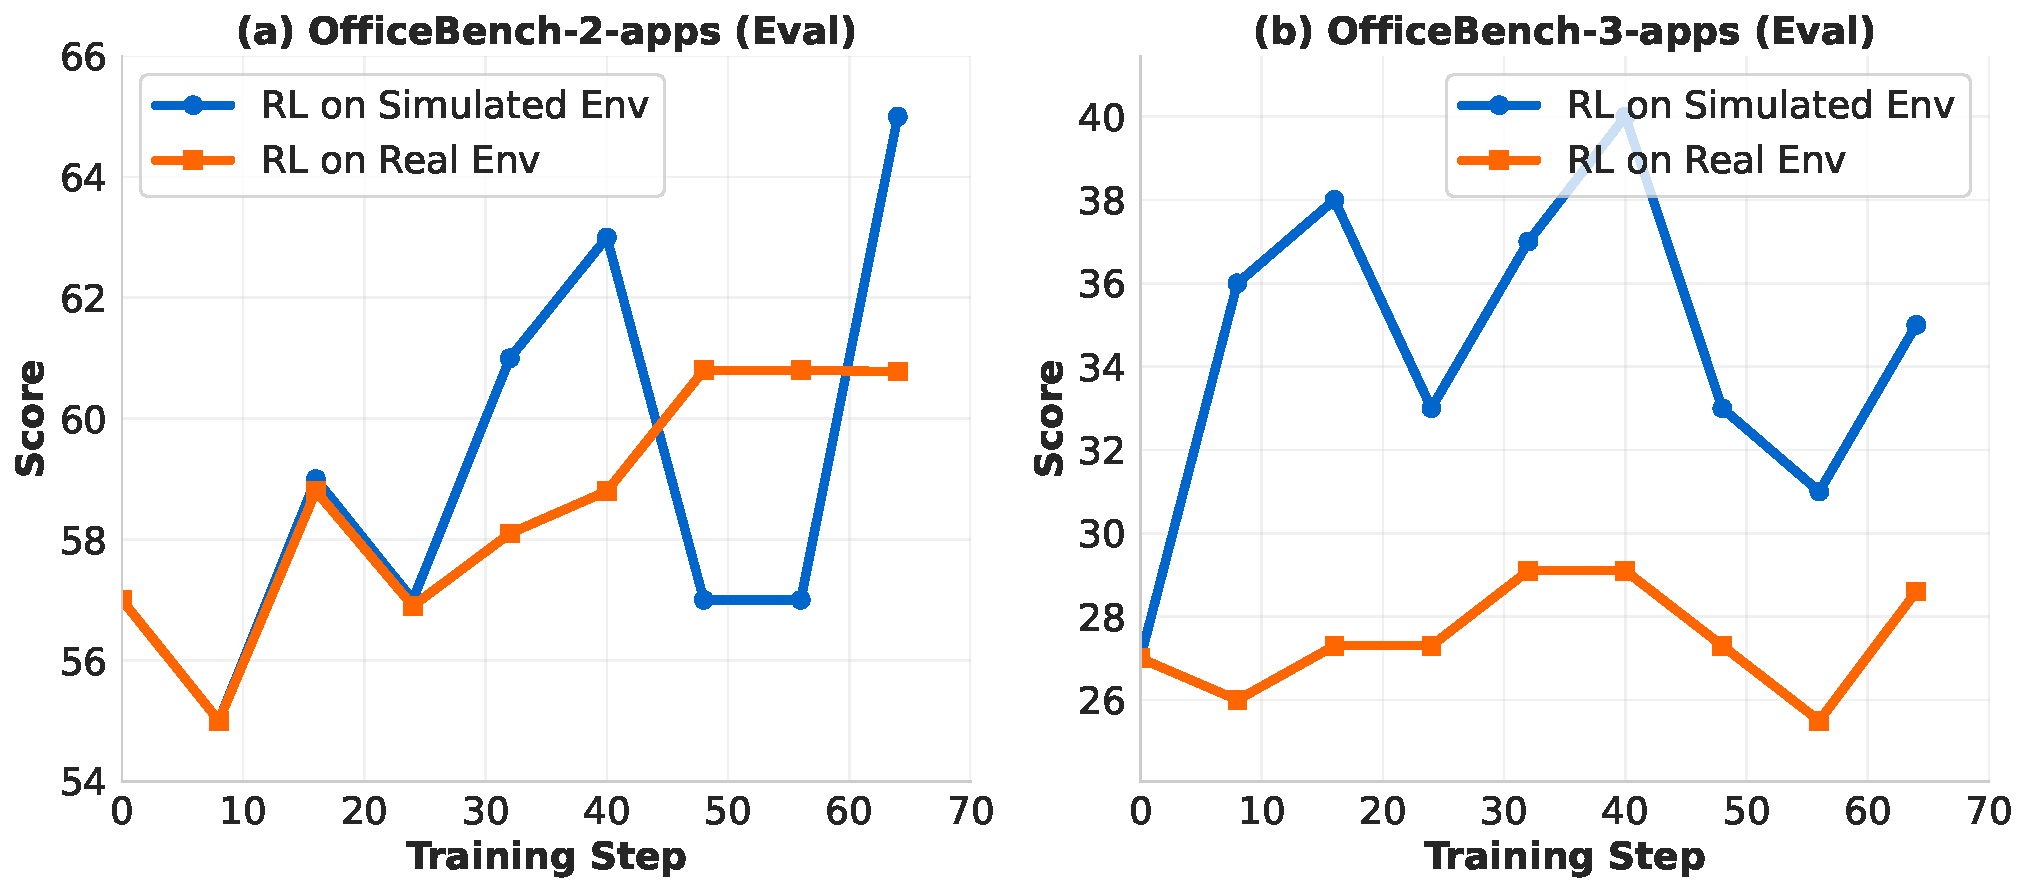
\includegraphics[width=0.7\textwidth]{figs/officebench_rl_training_curve.pdf}
    \caption{Performance of RL on simulated environment and real environment across different training steps for OfficeBench.}
    \label{fig:officebench_rl_training_curve}
\end{figure*}


\begin{figure*}[htbp]
    \centering
    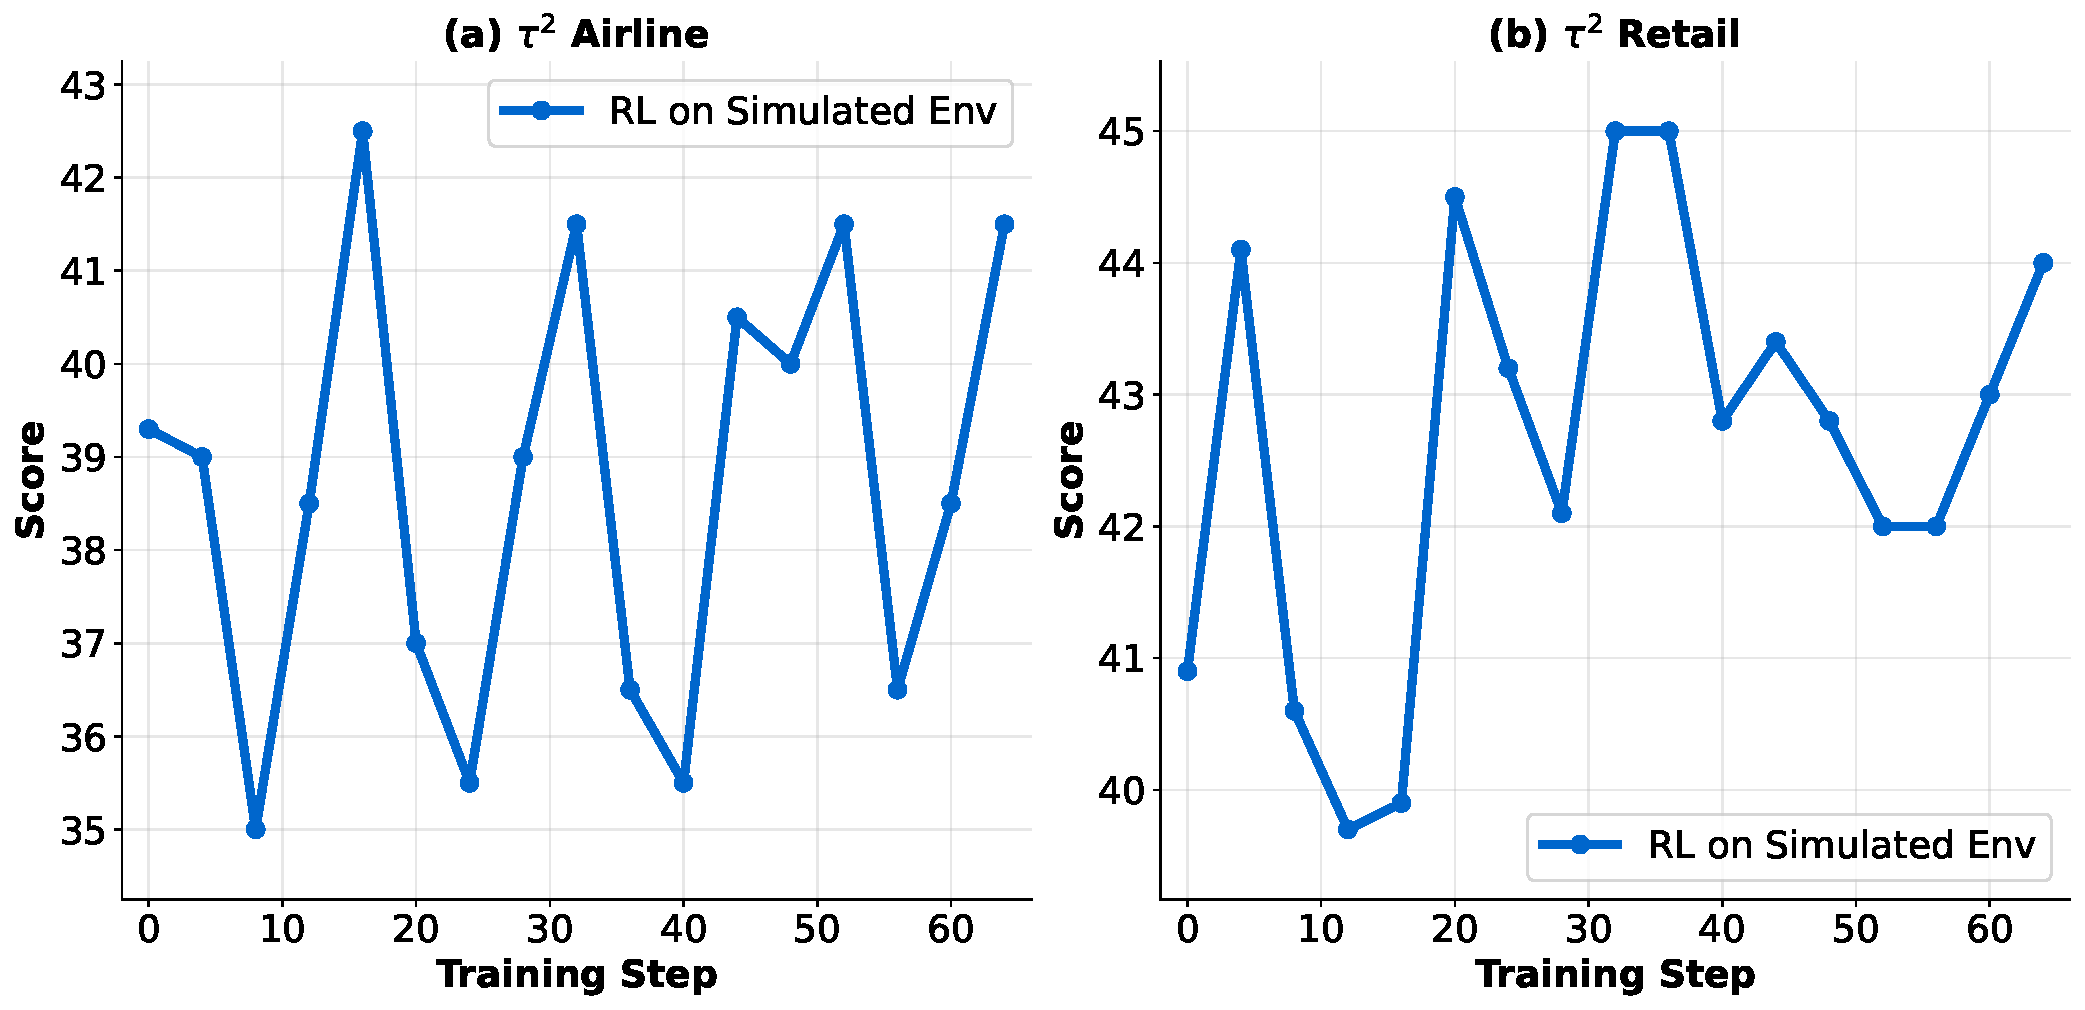
\includegraphics[width=0.7\textwidth]{figs/tau2_rl_training_curve.pdf}
    \caption{Performance of RL on simulated environment across different training steps for APIGen-MT.}
    \label{fig:tau2_rl_training_curve}
\end{figure*}
We present the experimental results for the RL performance on the simulated environment for OfficeBench and APIGen-MT across training steps, as depicted in Figure \ref{fig:officebench_rl_training_curve} and \ref{fig:tau2_rl_training_curve}. The evaluation performance on the OfficeBench 2-apps and 3-apps tasks demonstrates improvement, with 2-apps scores rising steadily from around 57.8 to approximately 64.7, and 3-apps scores increasing from 27.3 to 34.5. We can find that for the 3-apps performance RL on simulated environment is always better than real environment. RL on APIGen-MT also slightly improves performance on $\tau^2$-Bench. 
